\chapter{Preliminary Analysis of a Rocket}
The following chapter describes the functionality and structure behind a rocket. The goal is to determine which factors that leads to instability in flight and launch of a rocket. 
\bigbreak

The rocket which will described is based on:
\begin{itemize}[noitemsep]
\item A payload system.
\item A guidance system to control the rocket.
\item A propulsion system to launch the rocket with. 
\item Structure system consisting of nose cone, frame and fins.
\end{itemize}    

\begin{figure}[htbp]
	\centering
 	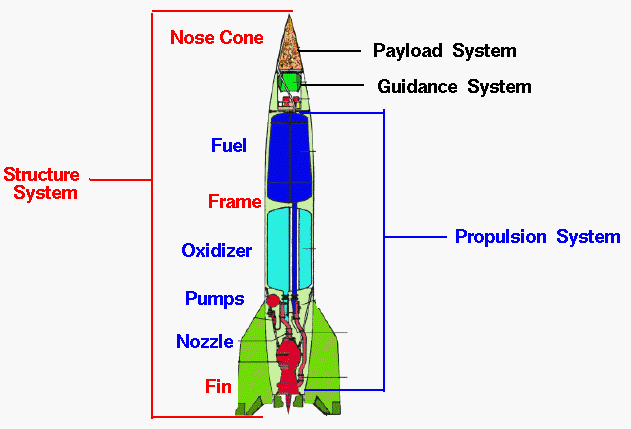
\includegraphics[width=0.7\textwidth]{figures/RocketStructure.png} 
 	\caption{Basic structure of a rocket.}
 	\label{fig:RocketStructure}
\end{figure}
%https://spaceflightsystems.grc.nasa.gov/education/rocket/rockpart.html


\section{Stability of a Rocket}
Describe why stability is important to for a rocket. 
\section{Mechanical System of a Rocket}
Input/output relation of a rocket.
\section{The Inverse Pendulum}
relate the rocket model to a Inverse Pendulum